\documentclass[11pt, a4paper]{article}
\usepackage{graphicx}
\usepackage{amsmath}
\usepackage[margin=0.6in]{geometry}
\usepackage{listings}
\usepackage{float}

\title{\centering \textbf{EE2703: Applied Programming Lab\\Week3: Fitting Data to Models }} % Title
\author{\textbf{Niyas Mon P | EE20B094}} % Author name
\date{\today} % Date for the report

\begin{document}
    \maketitle{} % Insert the title, author and date

    \section{Objectives}
        \begin{itemize}
            \item Make the best model/estimate for the data given
            \item Observe on how error is varied with respect to the noise in the data.
        \end{itemize}
    \section{Theory}
        The file “generate data.py” will generate a set of data with different levels of noise in it as follows:
        \begin{equation}
                f(t) = 1.05J_2(t)-0.105t+n(t)
            \end{equation}
        where n(t) is the amounts of noise according to the following distribution:
        \begin{equation}
                P(n(t)|\sigma)=\frac{1}{\sqrt{2\pi\sigma^2}}e^{-\frac{n(t)^2}{2\sigma^2}} \label{eq1}
            \end{equation}
        Now we have to fit the datas in "fitting.dat" using the following model.Here, we have to find the values of A and B which would best fit using least square error
        \begin{equation}
            g(t;A,B) = AJ_2(t)+Bt
        \end{equation}
        while the true values of A and B are:
        \begin{equation}
            A = 1.05 , B = -0.105
        \end{equation}
        \\
        To solve this first we make a matrix \textit{M} whose columns are Bassel function \textit{J(t)} and time \textit{t} and vector \textit{P} for the values of A and B \\
                \begin{equation}
                \textit{g(t;A,B)} = 
            \left(\begin{matrix}
            J_2(t_1) & t_1\\
            J_2(t_2) & t_2\\
            ... & ...\\
            J_2(t_m) & t_m\\
            \end{matrix}\right)
            .
            \left(\begin{matrix}
            A\\
            B\\
            \end{matrix}\right)
             = \textit{M.p}
        \end{equation}

        We are also doing contour plot for different values of A and B for the first data. For \textit{A =0, 0.1, ..., 2} and \textit{B =−0.2,−0.19,...0} we calculate:
        \begin{equation}
           \epsilon_{ij} = \frac{1}{101}\sum_{k=0}^{101}(f(t_k) - g(t_k, A_i, B_j))^2 
        \end{equation}

        And finally we are finally plotting errors in values of \textit{A} and \textit{B} in normal and log-log scale

    \section{Plots}
        \subsection{Extraction and Plotting of noisy data}
        
            The data in the fitting.dat file is plotted:
            
            \begin{figure}[H]
                \centering
                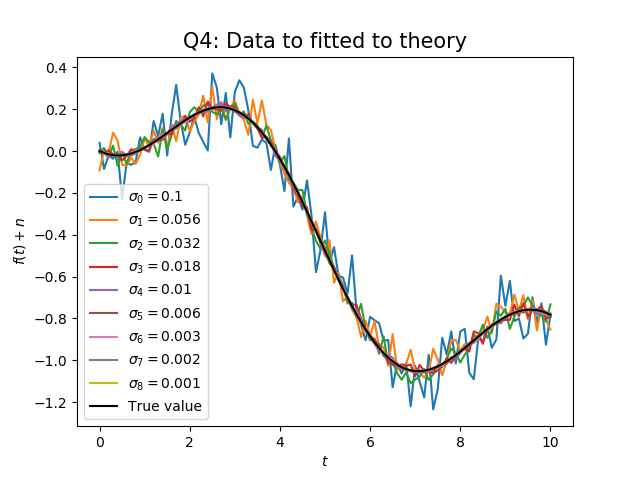
\includegraphics[scale=0.5]{q4_plot.png}
                \caption{Noisy Data and True Data}
                \label{fig:noisyAndTrue}
            \end{figure}
    \subsection{Plotting Errorbars}
            Now we are plotting first data in "fitting.dat" file with error bars with every fifth data in it along with true values to compare
            \begin{figure}[H]
                \centering
                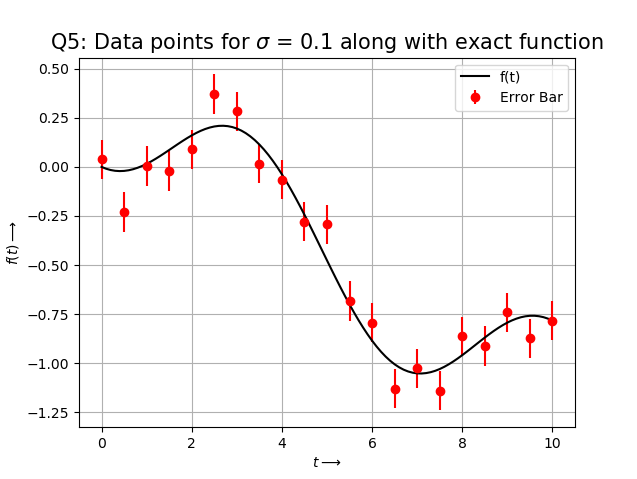
\includegraphics[scale=0.5]{q5_plot.png}
                \caption{Noisy Data with Errorbar}
                \label{fig:noiseError}
            \end{figure}
        \\
        \\
        \\
        
            

        \subsection{Finding the best fit for the data}
            From the data, we can say that the data can be fitted into a function of the form:
            \begin{equation}
                g(t, A, B) = AJ_2(t)+Bt
            \end{equation}
            
            where the coefficients $A$ and $B$ are  to be found.\\

            To find the coefficients $A$ and $B$, we are finding the mean square error between the function and the data for a range of values of \textit{A} and \textit{B},given by:
            \begin{equation}
           \epsilon_{ij} = \frac{1}{101}\sum_{k=0}^{101}(f(t_k) - g(t_k, A_i, B_j))^2 
        \end{equation}
        and plotting the contour line and finding the minimum for the best fit as follows:
        
            \begin{figure}[H]
                \centering
                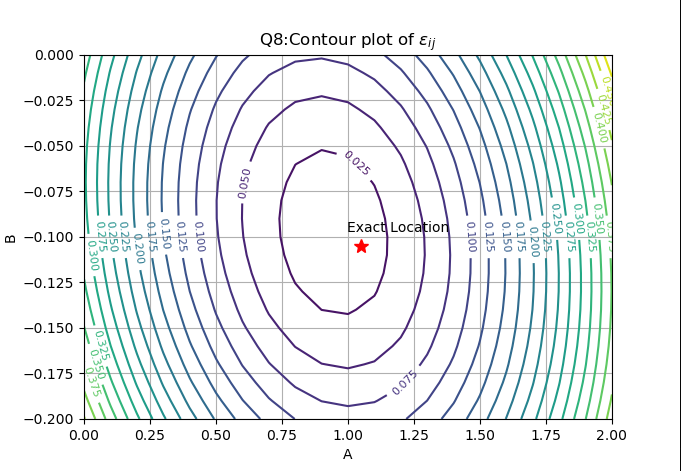
\includegraphics[scale=0.5]{q8_plot.png}  % Mention the image name within the curly braces. Image should be in the same folder as the tex file.
                \caption{Contour Plot of $\epsilon_{ij}$}
                \label{fig:contourPlot}
            \end{figure}

            The minima occur at \textbf{A = 1.05 and B = -0.105}






           

        \subsection{Error plots: Variation of error with $\sigma$}
        
            The plot of error in our approximation of A and B using the \texttt{lstsq} function with the standard deviation of the noise in the data
            \begin{figure}[H]
                \centering
                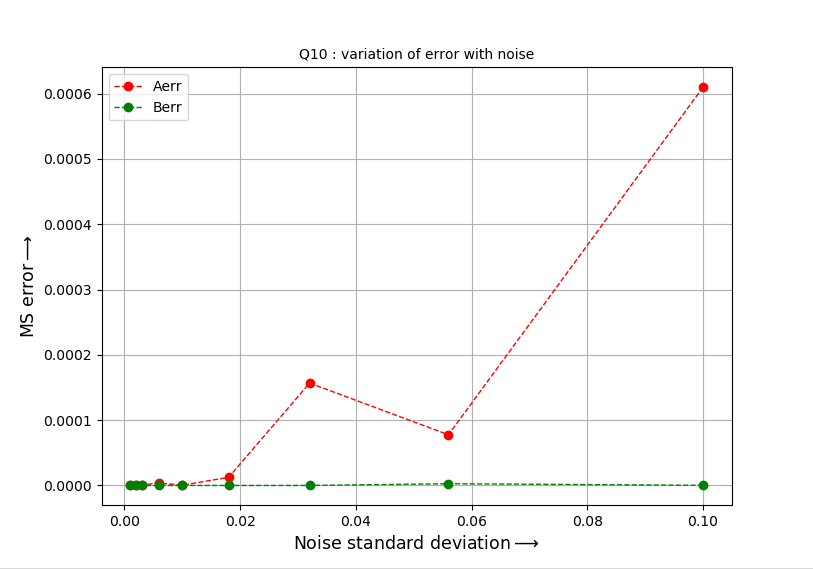
\includegraphics[scale=0.5]{q10_plot.png}  % Mention the image name within the curly braces. Image should be in the same folder as the tex file.
                \caption{Mean Squared Error vs Standard Deviation}
                \label{fig:errorSTD}
            \end{figure}

            Now we are plotting same info in log-log scale 
            \begin{figure}[H]
                \centering
                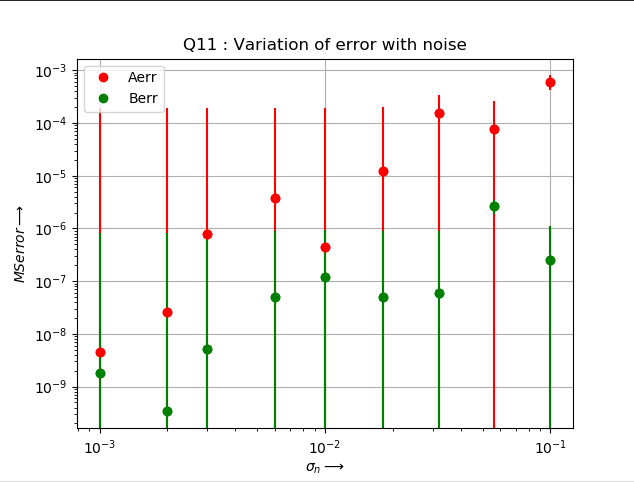
\includegraphics[scale=0.5]{q11_plot.png}  % Mention the image name within the curly braces. Image should be in the same folder as the tex file.
                \caption{MS Error vs Standard Deviation (\texttt{loglog}) Plot}
                \label{fig:errorSTDloglog}
            \end{figure}

            We can see an approximately linear relation between $\sigma_n$ and $\epsilon$.

    \section{Conclusions}
    \begin{itemize}
    \item In the contour plot, we can see that the MS error of the data converges to the
    true values of A and B and minimizing it using the least squares method we obtain a good estimation
    \item The value of B parameter changes very slowly compared to value of A in the normal
    scale but both A and b changes almost linearly with standard deviation in the logarithmic scale.
    \end{itemize}
    
\end{document}

